% TEXTALLION
% https://bitbucket.org/farvardin/textallion
% \LaTeX template 

\documentclass[openany]{book} % openany to remove the blank pages
% use report instead of article so you can use the "chapter"
%\documentclass[oneside]{book}
%\documentclass{article}
%\documentclass[twoside]{article}
%\noitemsep ?
% book = margins are shifted
% article = no shift for margins

\usepackage[activate={true,nocompatibility},final,tracking=true,kerning=true,spacing=true,factor=1100,stretch=10,shrink=10]{microtype}
% activate={true,nocompatibility} - activate protrusion and expansion
% final - enable microtype; use "draft" to disable
% tracking=true, kerning=true, spacing=true - activate these techniques
% factor=1100 - add 10% to the protrusion amount (default is 1000)
% stretch=10, shrink=10 - reduce stretchability/shrinkability (default is 20/20)

\flushbottom
\uchyph=0

\usepackage[pdftex]{graphicx}


\usepackage{paralist} % needed for compact lists
\usepackage[normalem]{ulem} % needed by strike
%  %hyperref defined elsewhere
\usepackage[utf8]{inputenc}  % char encoding
\usepackage{../includes/sample}  % user defined

%todo: check this:
\usepackage[protrusion=true,expansion=true]{microtype}


%---------------- Author & Metatags ------------------------------------

\def\DOCUMENTxTITLE{Textallion - Samples} % Titre of the document
\def\PDFAUTHOR{Various Authors}      % Authors
\def\PDFTITLE{\DOCUMENTxTITLE}      % copy of Titre of the document
\def\PDFSUBJECT{Novel, poetry, prosa} % Subjet
\def\PDFKEYWORDS{Novel, poetry, prosa}   % keywords, tags
\def\PDFCREATOR{Textallion, txt2tags, PdfTeX}   % Sofware which made this document
\def\PDFPRODUCER{Textallion}         % Compagny which made the software

% 

\usepackage[english,frenchb,francais]{babel}  
\usepackage[T1]{tipa}                       % additionnal fonts
\usepackage[\DEFAULTxFONTxSIZE pt]{extsizes} 
\usepackage[cm]{aeguill}                    % French guillemets
\usepackage[\SIZExOFxPAPER, \ORIENTATIONxOFxPAPER, total={\WIDTHxOFxTEXT mm,\HEIGHTxOFxTEXT mm},\GEOMETRYxADDITIONALxOPTION]{geometry}       % paper and text size


\usepackage{..//core/textallion}  % basic \LaTeX definitions for textallion

\def\MYxFONT{\rm}   % For correcting footers
\def\MYxFONTxMONO{}   % For correcting code area

%
% ------------ FONTS ---------------------------------------------------
\renewcommand{\rmdefault}{\DEFAULTxFONT} 
%



\title{Textallion, some examples}
\begin{document} \renewcommand*{\labelitemi}{$\bullet$} \renewcommand*{\labelitemii}{$\circ$} \renewcommand*{\labelitemiii}{$\cdot$} \renewcommand*{\labelitemiv}{$\diamond$}

\raggedbottom % avoid vertical jutification

\maketitle
% remove first page numbering on the cover
\thispagestyle{empty}
%\setcounter{page}{0}

\clearpage

%\pagestyle{headings} % page numbers_
%\pagenumbering{roman} % Roman numerals
%\setcounter{page}{2}

\tableofcontents
\clearpage

\hypertarget{toc1}{}
\pagebreak[\PAGExBREAKxPOLICY]
\part{Sample texts in English}

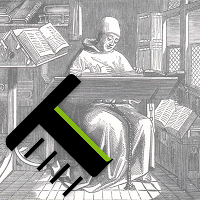
\includegraphics{../media/logo_textallion.png}

Here are some document examples for Textallion...

\begin{compactenum}
\item There are some poetry
\item Some prose as well
\item And some random stuffs
\end{compactenum}

\textit{See \href{../docs/documentation\_en.html}{documentation\_en.html} for the English manual.}

\hypertarget{toc2}{}
\pagebreak[\PAGExBREAKxPOLICY]
\chapter{Poetry}

\hypertarget{toc3}{}
\pagebreak[\PAGExSUBxBREAKxPOLICY]
\section{Gil-galad}

\textit{by JRR Tolkien}

\begin{center}
            \lunep
\par\noindent Gil-galad was an Elven-king.
\par\noindent Of him the harpers sadly sing:
\par\noindent The last whose realm was fair and free
\par\noindent Between the mountains and the sea.
            \lunefull
\par\noindent His sword was long, his lance was keen.
\par\noindent His shining helm afar was seen.
\par\noindent The countless stars of heaven's field
\par\noindent Were mirrored in his silver shield.
            \soleil
\par\noindent But long ago he rode away,
\par\noindent And where he dwelleth none can say.
\par\noindent For into darkness fell his star;
\par\noindent In Mordor, where the shadows are.
            \luned
\end{center}

\bigskip

\hypertarget{toc4}{}
\pagebreak[\PAGExSUBxBREAKxPOLICY]
\section{De Profundis}

\textit{by Christina Rossetti (1830-1894)}

\begin{center}

\par\noindent Oh why is heaven built so far,
\par\noindent Oh why is earth set so remote?
\par\noindent I cannot reach the nearest star
\par\noindent That hangs afloat.

	\begin{quotation}
		\begin{quotation}
			\begin{quotation}
 \newline
			\end{quotation}
		\end{quotation}
	\end{quotation}

\par\noindent I would not care to reach the moon,
\par\noindent One round monotonous of change;
\par\noindent Yet even she repeats her tune
\par\noindent Beyond my range.
             \newline
\par\noindent I never watch the scatter'd fire
\par\noindent Of stars, or sun's far-trailing train,
\par\noindent But all my heart is one desire,
\par\noindent And all in vain:
             \newline
\par\noindent For I am bound with fleshly bands,
\par\noindent Joy, beauty, lie beyond my scope;
\par\noindent I strain my heart, I stretch my hands,
\par\noindent And catch at hope.

\troisetoiles

\end{center}

\hypertarget{toc5}{}
\pagebreak[\PAGExBREAKxPOLICY]
\chapter{Prose}

\hypertarget{toc6}{}
\pagebreak[\PAGExSUBxBREAKxPOLICY]
\section{The Great God Pan}

\textit{Arthur Machen}

\parag

\bigskip

"Herbert! Good God! Is it possible?"

\bigskip
"Yes, my name's Herbert. I think I know your face, too, but I don't remember your name. My memory is very queer."

\bigskip
"Don't you recollect Villiers of Wadham?"

\bigskip
"So it is, so it is. I beg your pardon, Villiers, I didn't think I was begging of an old college friend. Good-night."

\bigskip
"My dear fellow, this haste is unnecessary. My rooms are close by, but we won't go there just yet. Suppose we walk up Shaftesbury Avenue a little way? But how in heaven's name have you come to this pass, Herbert?"

\bigskip
"It's a long story, Villiers, and a strange one too, but you can hear it if you like."

\bigskip
"Come on, then. Take my arm, you don't seem very strong."

\bigskip
The ill-assorted pair moved slowly up Rupert Street; the one in dirty, evil-looking rags, and the other attired in the regulation uniform of a man about town, trim, glossy, and eminently well-to-do. Villiers had emerged from his restaurant after an excellent dinner of many courses, assisted by an ingratiating little flask of Chianti, and, in that frame of mind which was with him almost chronic, had delayed a moment by the door, peering round in the dimly-lighted street in search of those mysterious incidents and persons with which the streets of London teem in every quarter and every hour. Villiers prided himself as a practised explorer of such obscure mazes and byways of London life, and in this unprofitable pursuit he displayed an assiduity which was worthy of more serious employment. Thus he stood by the lamp-post surveying the passers-by with undisguised curiosity, and with that gravity known only to the systematic diner, had just enunciated in his mind the formula: "London has been called the city of encounters; it is more than that, it is the city of Resurrections," when these reflections were suddenly interrupted by a piteous whine at his elbow, and a deplorable appeal for alms. He looked around in some irritation, and with a sudden shock found himself confronted with the embodied proof of his somewhat stilted fancies. There, close beside him, his face altered and disfigured by poverty and disgrace, his body barely covered by greasy ill-fitting rags, stood his old friend Charles Herbert, who had matriculated on the same day as himself, with whom he had been merry and wise for twelve revolving terms. Different occupations and varying interests had interrupted the friendship, and it was six years since Villiers had seen Herbert; and now he looked upon this wreck of a man with grief and dismay, mingled with a certain inquisitiveness as to what dreary chain of circumstances had dragged him down to such a doleful pass. Villiers felt together with compassion all the relish of the amateur in mysteries, and congratulated himself on his leisurely speculations outside the restaurant.

\bigskip
They walked on in silence for some time, and more than one passer-by stared in astonishment at the unaccustomed spectacle of a well-dressed man with an unmistakable beggar hanging on to his arm, and, observing this, Villiers led the way to an obscure street in Soho. Here he repeated his question. 

\parag 

\hypertarget{toc7}{}
\pagebreak[\PAGExSUBxBREAKxPOLICY]
\section{The Raven}

\textit{Poe}
\textit{1845}

\bigskip

\par\noindent 

\lettrine[lines=\INITIALxLETTERxSIZE, lhang=0.33, loversize=0.25]{O}{nce} upon a midnight dreary, while I pondered, weak and weary,
\par\noindent Over many a quaint and curious volume of forgotten lore,
\par\noindent While I nodded, nearly napping, suddenly there came a tapping,
\par\noindent As of some one gently rapping, rapping at my chamber door.
\par\noindent “ T’ is some visitor”, I muttered, “tapping at my chamber door~—
    Only this, and nothing more.”

\bigskip
\par\noindent And the silken sad uncertain rustling of each purple curtain
\par\noindent Thrilled me — filled me with fantastic terrors never felt before;
\par\noindent So that now, to still the beating of my heart, I stood repeating,
\par\noindent “ T’ is some visitor entreating entrance at my chamber door~—
\par\noindent Some late visitor entreating entrance at my chamber door;~—
     This it is, and nothing more.”

\bigskip
\par\noindent Presently my soul grew stronger; hesitating then no longer,
\par\noindent “Sir,” said I, “or Madam, truly your forgiveness I implore;
\par\noindent But the fact is I was napping, and so gently you came rapping,
\par\noindent And so faintly you came tapping, tapping at my chamber door,
\par\noindent That I scarce was sure I heard you” —~here I opened wide the door;~—
     Darkness there, and nothing more.

\bigskip
\par\noindent Deep into that darkness peering, long I stood there wondering, fearing,
\par\noindent Doubting, dreaming dreams no mortal ever dared to dream before;
\par\noindent But the silence was unbroken, and the stillness gave no token,
\par\noindent And the only word there spoken was the whispered word, “Lenore?”
\par\noindent This I whispered, and an echo murmured back the word, “Lenore!”~—
     Merely this, and nothing more.

\bigskip
\par\noindent Back into the chamber turning, all my soul within me burning,
\par\noindent Soon again I heard a tapping somewhat louder than before.
\par\noindent “Surely,” said I, “surely that is something at my window lattice:
\par\noindent Let me see, then, what thereat is, and this mystery explore~—
\par\noindent Let my heart be still a moment and this mystery explore;~—
     ’Tis the wind and nothing more.”

\bigskip
\par\noindent Open here I flung the shutter, when, with many a flirt and flutter,
\par\noindent In there stepped a stately raven of the saintly days of yore;
\par\noindent Not the least obeisance made he; not a minute stopped or stayed he;
\par\noindent But, with mien of lord or lady, perched above my chamber door~—
\par\noindent Perched upon a bust of Pallas just above my chamber door~—
     Perched, and sat, and nothing more.

\bigskip
\par\noindent Then this ebony bird beguiling my sad fancy into smiling,
\par\noindent By the grave and stern decorum of the countenance it wore.
\par\noindent “Though thy crest be shorn and shaven, thou,” I said, “art sure no craven,
\par\noindent Ghastly grim and ancient raven wandering from the Nightly shore~—
\par\noindent Tell me what thy lordly name is on the Night’s Plutonian shore!”
     Quoth the Raven, “Nevermore.”

\bigskip
\par\noindent Much I marveled this ungainly fowl to hear discourse so plainly,
\par\noindent Though its answer little meaning — little relevancy bore;
\par\noindent For we cannot help agreeing that no living human being
\par\noindent Ever yet was blest with seeing bird above his chamber door~—
\par\noindent Bird or beast upon the sculptured bust above his chamber door,
     With such name as “Nevermore.”

\bigskip
\par\noindent But the raven, sitting lonely on the placid bust, spoke only
\par\noindent That one word, as if his soul in that one word he did outpour.
\par\noindent Nothing further then he uttered — not a feather then he fluttered~—
\par\noindent Till I scarcely more than muttered, “other friends have flown before~—
\par\noindent On the morrow he will leave me, as my hopes have flown before.”
     Then the bird said, “Nevermore.”

\bigskip
\par\noindent Startled at the stillness broken by reply so aptly spoken,
\par\noindent “Doubtless,” said I, “what it utters is its only stock and store,
\par\noindent Caught from some unhappy master whom unmerciful Disaster
\par\noindent Followed fast and followed faster till his songs one burden bore~—
\par\noindent Till the dirges of his Hope that melancholy burden bore
     Of ’Never — nevermore’.”

\bigskip
\par\noindent But the Raven still beguiling all my sad soul into smiling,
\par\noindent Straight I wheeled a cushioned seat in front of bird, and bust and door;
\par\noindent Then upon the velvet sinking, I betook myself to linking
\par\noindent Fancy unto fancy, thinking what this ominous bird of yore~—
\par\noindent What this grim, ungainly, ghastly, gaunt and ominous bird of yore
     Meant in croaking “Nevermore.”

\bigskip
\par\noindent This I sat engaged in guessing, but no syllable expressing
\par\noindent To the fowl whose fiery eyes now burned into my bosom’s core;
\par\noindent This and more I sat divining, with my head at ease reclining
\par\noindent On the cushion’s velvet lining that the lamplight gloated o’er,
\par\noindent But whose velvet violet lining with the lamplight gloating o’er,
     She shall press, ah, nevermore!

\bigskip
\par\noindent Then methought the air grew denser, perfumed from an unseen censer
\par\noindent Swung by Seraphim whose footfalls tinkled on the tufted floor.
\par\noindent “Wretch,” I cried, “thy God hath lent thee — by these angels he hath sent thee
\par\noindent Respite — respite and nepenthe, from thy memories of Lenore
\par\noindent Quaff, oh quaff this kind nepenthe and forget this lost Lenore!”
     Quoth the Raven, “Nevermore.”

\bigskip
\par\noindent “Prophet!” said I, “thing of evil! — prophet still, if bird or devil!~—
\par\noindent Whether Tempter sent, or whether tempest tossed thee here ashore,
\par\noindent Desolate yet all undaunted, on this desert land enchanted —
\par\noindent On this home by horror haunted — tell me truly, I implore —
\par\noindent Is there — is there balm in Gilead? — tell me — tell me, I implore!”
     Quoth the Raven, “Nevermore.”

\bigskip
\par\noindent “Prophet!” said I, “thing of evil — prophet still, if bird or devil!
\par\noindent By that Heaven that bends above us — by that God we both adore~—
\par\noindent Tell this soul with sorrow laden if, within the distant Aidenn,
\par\noindent It shall clasp a sainted maiden whom the angels name Lenore —
\par\noindent Clasp a rare and radiant maiden whom the angels name Lenore.”
     Quoth the Raven, “Nevermore.”

\bigskip
\par\noindent “Be that word our sign in parting, bird or fiend,” I shrieked, upstarting~—
\par\noindent “Get thee back into the tempest and the Night’s Plutonian shore!
\par\noindent Leave no black plume as a token of that lie thy soul hath spoken!
\par\noindent Leave my loneliness unbroken! — quit the bust above my door!
\par\noindent Take thy beak from out my heart, and take thy form from off my door!”
     Quoth the Raven, “Nevermore.”

\bigskip
\par\noindent And the Raven, never flitting, still is sitting, still is sitting
\par\noindent On the pallid bust of Pallas just above my chamber door;
\par\noindent And his eyes have all the seeming of a demon’s that is dreaming,
\par\noindent And the lamplight o’er him streaming throws his shadow on the floor;
\par\noindent And my soul from out that shadow that lies floating on the floor
     Shall be lifted — nevermore!

\parag 

\hypertarget{toc8}{}
\pagebreak[\PAGExBREAKxPOLICY]
\part{Examples de textes en français}

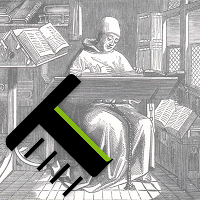
\includegraphics{../media/logo_textallion.png}

Voici quelques exemples de documents utilisant le TeXtallion...

\begin{compactenum}
\item Il y a de la poésie
\item un peu de prose
\item et divers styles de textes
\end{compactenum}

\textit{Voir \href{docs/documentation\_fr.html}{documentation\_fr.html} pour le manuel en français.}

\hypertarget{toc9}{}
\pagebreak[\PAGExBREAKxPOLICY]
\chapter{Exemple de poésie}

\hypertarget{toc10}{}
\pagebreak[\PAGExSUBxBREAKxPOLICY]
\section{Tristesses de la lune}

\textit{Baudelaire}

\begin{center}
              \lunep
\par\noindent Ce soir, la lune rêve avec plus de paresse;
\par\noindent Ainsi qu'une beauté, sur de nombreux coussins,
\par\noindent Qui d'une main distraite et légère caresse
\par\noindent Avant de s'endormir le contour de ses seins,
              \lunefull        
\par\noindent Sur le dos satiné des molles avalanches,
\par\noindent Mourante, elle se livre aux longues pâmoisons,
\par\noindent Et promène ses yeux sur les visions blanches
\par\noindent Qui montent dans l'azur comme des floraisons.
              \luned
\par\noindent Quand parfois sur ce globe, en sa langueur oisive,
\par\noindent Elle laisse filer une larme furtive,
\par\noindent Un poëte pieux, ennemi du sommeil,
              \soleil
\par\noindent Dans le creux de sa main prend cette larme pâle,
\par\noindent Aux reflets irisés comme un fragment d'opale,
\par\noindent Et la met dans son cœur loin des yeux du soleil.
              \luned
\end{center}

\hypertarget{toc11}{}
\pagebreak[\PAGExSUBxBREAKxPOLICY]
\section{Aux modernes}

\textit{Leconte de Lisle}

\begin{center}
\par\noindent Vous vivez lâchement, sans rêve, sans dessein,
\par\noindent Plus vieux, plus décrépits que la terre inféconde,
\par\noindent Châtrés dès le berceau par le siècle assassin
\par\noindent De toute passion vigoureuse et profonde.

\par\noindent Votre cervelle est vide autant que votre sein,
\par\noindent Et vous avez souillé ce misérable monde
\par\noindent D’un sang si corrompu, d’un souffle si malsain,
\par\noindent Que la mort germe seule en cette boue immonde.

\par\noindent Hommes, tueurs de Dieux, les temps ne sont pas loin
\par\noindent Où, sur un grand tas d’or vautrés dans quelque coin,
\par\noindent Ayant rongé le sol nourricier jusqu’aux roches

\par\noindent Ne sachant faire rien ni des jours ni des nuits,
\par\noindent Noyés dans le néant des suprêmes ennuis,
\par\noindent Vous mourrez bêtement en emplissant vos poches.
\end{center}

\troisetoiles

\hypertarget{toc12}{}
\pagebreak[\PAGExBREAKxPOLICY]
\chapter{Prose}

\hypertarget{toc13}{}
\pagebreak[\PAGExSUBxBREAKxPOLICY]
\section{Le Chat}

\textit{Théodore de Banville}
\textit{(1882)}

\bigskip


\lettrine[lines=\INITIALxLETTERxSIZE, lhang=0.33, loversize=0.25]{T}{out} animal est supérieur à l'homme par ce qu'il y a en lui de divin, c'est-à-dire par l'instinct. Or, de tous les animaux, le Chat est celui chez lequel l'instinct est le plus persistant, le plus impossible à tuer. Sauvage ou domestique, il reste lui-même, obstinément, avec une sérénité absolue, et aussi rien ne peut lui faire perdre sa beauté et sa grâce suprême. Il n'y a pas de condition si humble et si vile qui arrive à le dégrader, parce qu'il n'y consent pas, et qu'il garde toujours la seule liberté qui puisse être accordée aux créatures, c'est-à-dire la volonté et la résolution arrêtée d'être libre. Il l'est en effet, parce qu'il ne se donne que dans la mesure où il le veut, accordant ou refusant à son gré son affection et ses caresses, et c'est pourquoi il reste beau, c'est-à-dire semblable à son type éternel. Prenez deux Chats, l'un vivant dans quelque logis de grande dame ou de poète, sur les moelleux tapis, sur les divans de soie et les coussins armoriés, l'autre étendu sur le carreau rougi, dans un logis de vieille fille pauvre, ou pelotonné dans une loge de portière, eh bien~! tous deux auront au même degré la noblesse, le respect de soi-même, l'élégance à laquelle le Chat ne peut renoncer sans mourir.

\bigskip
En lisant le morceau si épouvantablement injuste que Buffon a consacré au Chat, on reconstruirait, si la mémoire en était perdue, tout ce règne de Louis XIV où l'homme se crut devenu soleil et centre du monde, et ne put se figurer que des milliers d'astres et d'étoiles avaient été jetés dans l'éther pour autre chose que pour son usage personnel. Ainsi le savant à manchettes, reprochant au gracieux animal de voler ce qu'il lui faut pour sa nourriture, semble supposer chez les Chats une notion exacte de la propriété et une connaissance approfondie des codes, qui par bonheur n'ont pas été accordées aux animaux. «~Ils n'ont, ajoute-t-il que l'apparence de l'attachement~; on le voit à leurs mouvements obliques, à leurs yeux équivoques~; ils ne regardent jamais en face la personne aimée~; soit défiance ou fausseté, ils prennent des détours pour en approcher, pour chercher des caresses auxquelles ils ne sont sensibles que pour le plaisir qu'elles leur font.~» O injuste grand savant que vous êtes~! Est-ce que nous cherchons, nous, les caresses pour le plaisir qu'elles ne nous font pas~? Vous dites que les yeux des Chats sont équivoques~! Relativement à quoi~? Si tout d'abord nous n'en pénétrons pas la subtile et profonde pensée, cela ne tient-il pas à notre manque d'intelligence et d'intuition~? Quant aux détours, eh~! mais le spirituel Alphonse Karr a adopté cette devise charmante : «~Je ne crains que ceux que j'aime,~» et, comme on le voit, le Chat, plein de prudence, l'avait adoptée avant lui.

\bigskip 
Sans doute, il se laisse toucher, caresser, tirer les poils, porter la tête en bas par les enfants, instinctifs comme lui~; mais il se défie toujours de l'homme, et c'est en quoi il prouve son profond bon sens. N'a-t-il pas sous les yeux l'exemple de ce Chien que le même Buffon met si haut, et ne voit-il pas par là ce que l'homme fait des animaux qui consentent à être ses serviteurs et se donnent à lui sans restriction, une fois pour toutes~? L'homme fait du Chien un esclave attaché, mis à la chaîne~; il lui fait traîner des carrioles et des voitures, il l'envoie chez le boucher chercher de la viande à laquelle il ne devra pas toucher. Il le réduit même à la condition dérisoire de porter les journaux dans le quartier~; il avait fait du Chien Munito un joueur de dominos, et pour peu il l'aurait réduit à exercer le métier littéraire, à faire de la copie, ce qui, pour un animal né libre sous les cieux, ma paraîtrait le dernier degré de l'abaissement. L'homme oblige le Chien à chasser pour lui, à ses gages et même sans gages~; le Chat préfère chasser pour son propre compte, et à ce sujet on l'appelle voleur, sous prétexte que les lapins et les oiseaux appartiennent à l'homme~; mais c'est ce qu'il faudrait démontrer. On veut lui imputer à crime ce qui fit la gloire de Nemrod et d'Hippolyte, et c'est ainsi que nous avons toujours deux poids inégaux, et deux mesures.

\parag 

\hypertarget{toc14}{}
\pagebreak[\PAGExSUBxBREAKxPOLICY]
\section{Une ville flottante}

\textit{Jules Verne (1871)}

«~Quel est cet homme~?

— Je ne sais, répondis-je.

--- Il me déplaît~!~» ajouta Fabian. Mettez deux navires en pleine mer, sans vent, sans courant, et ils finiront par s’accoster : Jetez deux planètes immobiles dans l’espace, et elles tomberont l’une sur l’autre. Placez deux ennemis au milieu d’une foule, et ils se rencontreront inévitablement. C’est fatal. Une question de temps, voilà tout. 

Le soir arrivé, le concert eut lieu selon le programme. Le grand salon rempli d’auditeurs, était brillamment éclairé. /.../

\textit{(extrait du chapitre 16)}

\hypertarget{toc15}{}
\pagebreak[\PAGExSUBxBREAKxPOLICY]
\section{Le Corbeau}

\textit{(Poe / Baudelaire)} \footnote{\MYxFONT Ce texte a été publié en 1845, et a été traduit ensuite en français par Baudelaire, ainsi que par Mallarmé. C'est la version de Baudelaire que nous vous livrons ici.}

\bigskip


\lettrine[lines=\INITIALxLETTERxSIZE, lhang=0.33, loversize=0.25]{U}{ne} fois, sur le minuit lugubre, pendant que je méditais, faible et fatigué, sur maint précieux et curieux volume d’une doctrine oubliée, pendant que je donnais de la tête, presque assoupi, soudain il se fit un tapotement, comme de quelqu’un frappant doucement, frappant à la porte de ma chambre. «~C’est quelque visiteur, – murmurai-je, – qui frappe à la porte de ma chambre~; ce n’est que cela et rien de plus.~»

\bigskip
Ah~! distinctement je me souviens que c’était dans le glacial décembre, et chaque tison brodait à son tour le plancher du reflet de son agonie. Ardemment je désirais le matin~; en vain m’étais-je efforcé de tirer de mes livres un sursis à ma tristesse, ma tristesse pour ma Lénore perdue, pour la précieuse et rayonnante fille que les anges nomment Lénore, – et qu’ici on ne nommera jamais plus.

\bigskip
Et le soyeux, triste et vague bruissement des rideaux pourprés me pénétrait, me remplissait de terreurs fantastiques, inconnues pour moi jusqu’à ce jour~; si bien qu’enfin pour apaiser le battement de mon cœur, je me dressai, répétant : «~C’est quelque visiteur attardé sollicitant l’entrée à la porte de ma chambre~; – c’est cela même, et rien de plus.~»

\bigskip
Mon âme en ce moment se sentit plus forte. N’hésitant donc pas plus longtemps : «~Monsieur, dis-je, ou madame, en vérité, j’implore votre pardon~; mais le fait est que je sommeillais et vous êtes venu frapper si doucement, si faiblement vous êtes venu frapper à la porte de ma chambre, qu’à peine étais-je certain de vous avoir entendu.~» Et alors j’ouvris la porte toute grande~; – les ténèbres, et rien de plus.

\bigskip
Scrutant profondément ces ténèbres, je me tins longtemps plein d’étonnement, de crainte, de doute, rêvant des rêves qu’aucun mortel n’a jamais osé rêver~; mais le silence ne fut pas troublé, et l’immobilité ne donna aucun signe, et le seul mot proféré fut un nom chuchoté : «~Lénore~!~» – C’était moi qui le chuchotais, et un écho à son tour murmura ce mot : «~Lénore~!~» Purement cela, et rien de plus.

\bigskip
Rentrant dans ma chambre, et sentant en moi toute mon âme incendiée, j’entendis bientôt un coup un peu plus fort que le premier. «~Sûrement, – dis-je, – sûrement, il y a quelque chose aux jalousies de ma fenêtre~; voyons donc ce que c’est, et explorons ce mystère. Laissons mon cœur se calmer un instant, et explorons ce mystère~; – c’est le vent, et rien de plus.~»

\bigskip
Je poussai alors le volet, et, avec un tumultueux battement d’ailes, entra un majestueux corbeau digne des anciens jours. Il ne fit pas la moindre révérence, il ne s’arrêta pas, il n’hésita pas une minute~; mais avec la mine d’un lord ou d’une lady, il se percha au-dessus de la porte de ma chambre~; il se percha sur un buste de Pallas juste au-dessus de la porte de ma chambre~; – il se percha, s’installa, et rien de plus.

\bigskip
Alors, cet oiseau d’ébène, par la gravité de son maintien et la sévérité de sa physionomie, induisant ma triste imagination à sourire : «~Bien que ta tête, – lui dis-je, – soit sans huppe et sans cimier, tu n’es certes pas un poltron, lugubre et ancien corbeau, voyageur parti des rivages de la nuit. Dis-moi quel est ton nom seigneurial aux rivages de la nuit plutonienne~!~» Le corbeau dit : «~Jamais plus~!~»

\bigskip
Je fus émerveillé que ce disgracieux volatile entendît si facilement la parole, bien que sa réponse n’eût pas un bien grand sens et ne me fût pas d’un grand secours~; car nous devons convenir que jamais il ne fut donné à un homme vivant de voir un oiseau au-dessus de la porte de sa chambre, un oiseau ou une bête sur un buste sculpté au-dessus de la porte de sa chambre, se nommant d’un nom tel que – Jamais plus~!

Mais le corbeau, perché solitairement sur le buste placide, ne proféra que ce mot unique, comme si dans ce mot unique il répandait toute son âme. Il ne prononça rien de plus~; il ne remua pas une plume, – jusqu’à ce que je me prisse à murmurer faiblement : «~D’autres amis se sont déjà envolés loin de moi~; vers le matin, lui aussi, il me quittera comme mes anciennes espérances déjà envolées.~» L’oiseau dit alors : «~Jamais plus~!~»

\bigskip
Tressaillant au bruit de cette réponse jetée avec tant d’à-propos : Sans doute, – dis-je, – ce qu’il prononce est tout son bagage de savoir, qu’il a pris chez quelque maître infortuné que le Malheur impitoyable a poursuivi ardemment, sans répit, jusqu’à ce que ses chansons n’eussent plus qu’un seul refrain, jusqu’à ce que le De profundis de son Espérance eût pris ce mélancolique refrain : «~Jamais – jamais plus~!~»

\bigskip
Mais le corbeau induisant encore toute ma triste âme à sourire, je roulai tout de suite un siège à coussins en face de l’oiseau et du buste et de la porte~; alors, m’enfonçant dans le velours, je m’appliquai à enchaîner les idées aux idées, cherchant ce que cet augural oiseau des anciens jours, ce que ce triste, disgracieux, sinistre, maigre et augural oiseau des anciens jours voulait faire entendre en croassant son – Jamais plus~!

\bigskip
Je me tenais ainsi, rêvant, conjecturant, mais n’adressant plus une syllabe à l’oiseau, dont les yeux ardents me brûlaient maintenant jusqu’au fond du cœur : je cherchai à deviner cela, et plus encore, ma tête reposant à l’aise sur le velours du coussin que caressait la lumière de la lampe, ce velours violet caressé par la lumière de la lampe que sa tête, à Elle, ne pressera plus, – ah~! jamais plus~!

\bigskip
Alors, il me sembla que l’air s’épaississait, parfumé par un encensoir invisible que balançaient les séraphins dont les pas frôlaient le tapis de ma chambre. «~Infortuné~! – m’écriai-je, – ton Dieu t’a donné par ses anges, il t’a envoyé du répit, du répit et du népenthès dans tes ressouvenirs de Lénore~! Bois, oh~! bois ce bon népenthès, et oublie cette Lénore perdue~!~» Le corbeau dit : «Jamais plus~!~»

\bigskip
«~Prophète~! – dis-je, – être de malheur~! oiseau ou démon~! mais toujours prophète~! que tu sois un envoyé du Tentateur, ou que la tempête t’ait simplement échoué, naufragé, mais encore intrépide, sur cette terre déserte, ensorcelée, dans ce logis par l’Horreur hanté, – dis-moi sincèrement, je t’en supplie, existe-t-il, existe-t-il ici un baume de Judée~? Dis, dis, je t’en supplie~!~» Le corbeau dit : «~Jamais plus~!~»

\bigskip
«~Prophète~! – dis-je, – être de malheur~! oiseau ou démon~! toujours prophète~! par ce ciel tendu sur nos têtes, par ce Dieu que tous deux nous adorons, dis à cette âme chargée de douleur si, dans le Paradis lointain, elle pourra embrasser une fille sainte que les anges nomment Lénore, embrasser une précieuse et rayonnante fille que les anges nomment Lénore.~» Le corbeau dit : «~Jamais plus~!~»

\bigskip
«~Que cette parole soit le signal de notre séparation, oiseau ou démon~! – hurlai-je en me redressant. – Rentre dans la tempête, retourne au rivage de la nuit plutonienne~; ne laisse pas ici une seule plume noire comme souvenir du mensonge que ton âme a proféré~; laisse ma solitude inviolée~; quitte ce buste au-dessus de ma porte~; arrache ton bec de mon cœur et précipite ton spectre loin de ma porte~!~» Le corbeau dit : «~Jamais plus~!~»

\bigskip
Et le corbeau, immuable, est toujours installé sur le buste pâle de Pallas, juste au-dessus de la porte de ma chambre~; et ses yeux ont toute la semblance des yeux d’un démon qui rêve~; et la lumière de la lampe, en ruisselant sur lui, projette son ombre sur le plancher~; et mon âme, hors du cercle de cette ombre qui gît flottante sur le plancher, ne pourra plus s’élever, – jamais plus~!
\parag 

\hypertarget{toc16}{}
\pagebreak[\PAGExBREAKxPOLICY]
\part{Diverses}

\textit{Some texts in other languages\footnote{\MYxFONT Not all unicode scripts are supported by xetex, but they should work in the html output.}.}



\lettrine[lines=\INITIALxLETTERxSIZE, lhang=0.33, loversize=0.25]{F}{jölnir} sonur Yngvifreys réð þá fyrir Svíum og Uppsalaauð. Hann var ríkur og ársæll og friðsæll. Þá var Frið-Fróði að Hleiðru. Þeirra í millum var heimboð og vingan. Þá er Fjölnir fór til Fróða á Selund þá var þar fyrir búin mikil veisla og boðið til víða um lönd. 

\bigskip

\begin{multicols}{2}

Fróði átti mikinn húsabæ. Þar var gert ker mikið margra alna hátt og okað með stórum timburstokkum. Það stóð í undirskemmu en loft var yfir uppi og opið gólfþilið svo að þar var niður hellt leginum en kerið blandið fullt mjaðar. Þar var drykkur furðu sterkur. 
Um kveldið var Fjölni fylgt til herbergis í hið næsta loft og hans sveit með honum. 

\end{multicols}

\bigskip

Um nóttina gekk hann út í svalar að leita sér staðar. Var hann svefnær og dauðadrukkinn. En er hann snerist aftur til herbergis þá gekk hann fram eftir svölunum og til annarra loftdura og þar inn, missti þá fótum og féll í mjaðarkerið og týndist þar.  
\par\noindent \aldineb 



\lettrine[lines=\INITIALxLETTERxSIZE, lhang=0.33, loversize=0.25]{L}{orem} ipsum dolor sit amet, consectetur adipisicing elit, sed do eiusmod tempor incididunt ut labore et dolore magna aliqua. Ut enim ad minim veniam, quis nostrud exercitation ullamco laboris nisi ut aliquip ex ea commodo consequat. Duis aute irure dolor in reprehenderit in voluptate velit esse cillum dolore eu fugiat nulla pariatur. Excepteur sint occaecat cupidatat non proident, sunt in culpa qui officia deserunt mollit anim id est laborum.

\bigskip

\begin{multicols}{3}

Lorem ipsum dolor sit amet, consectetur adipisicing elit, sed do eiusmod tempor incididunt ut labore et dolore magna aliqua. Ut enim ad minim veniam, quis nostrud exercitation ullamco laboris nisi ut aliquip ex ea commodo consequat. 

\bigskip

Duis aute irure dolor in reprehenderit in voluptate velit esse cillum dolore eu fugiat nulla pariatur. 

\end{multicols}

Excepteur sint occaecat cupidatat non proident, sunt in culpa qui officia deserunt mollit anim id est laborum.

«~Être moderne ne consiste pas à chercher quelque chose en dehors de tout ce qui a été fait. Il ne s'agit au contraire que de coordonner tout ce que les âges précédents nous ont apporté pour faire voir comment notre siècle a accepté cet héritage et comment il en use~». -- Gustave Moreau\footnote{\MYxFONT Peintre symboliste du 19ème siècle}

\par\noindent \parag 

\troisetoiles

\hypertarget{toc17}{}
\pagebreak[\PAGExBREAKxPOLICY]
\part{More tests}

\hypertarget{toc18}{}
\pagebreak[\PAGExBREAKxPOLICY]
\chapter{My Subtitle 1}

\begin{exergue}{Platon}
Si tu veux contrôler le peuple commence par contrôler sa musique.
\end{exergue}

\begin{exergue}{}
Quand l'achat et la vente sont contrôlés par la législation, les premières choses qui s'achètent et se vendent sont les législateurs.
\\[\EXERGUExAUTHORxSPACE pt] \EXERGUExSIZE \EXERGUExAUTHORxSHAPE {Patrick Jake O'Rourke} 
\end{exergue}

Some examples:

A paragraph with \textbf{bold}, \textit{italic} and \sout{strike}.
You can even \underline{underline your docs}!

And use \textbf{\textit{bold and italic}} 
or \textit{\textbf{italic and bold}} 

Here is a nice pic: [\href{http://txt2tags.sourceforge.net/img/t2tgems.png}{http://txt2tags.sourceforge.net/img/t2tgems.png}]

And a \href{http://txt2tags.sf.net}{link to a cool website}!

A table : 

\begin{center}\begin{longtabu}{|l|l|r|}
\hline \textbf{Name} & \textbf{Age} & \textbf{Gender} \\
\hline John & \multicolumn{1}{|c|}{33} & Male \\
\hline Mary & \multicolumn{1}{|c|}{19} & Female \\
\hline \end{longtabu}\end{center}

\begin{spverbatim}
A verbatim line
\end{spverbatim}

A raw line 

And it's working for \texttt{special code} like this.

\begin{spverbatim}
Unfortunately I can't color this verbatim content yet.
\end{spverbatim}

\begin{sourcecode}{
Test code source.

And a new line to test again.
And again...

And a new line to test again.
And a new line to test again.
}\end{sourcecode}

Raw area test

\href{mailto:username@example.com}{test email}

\hypertarget{toc19}{}
\pagebreak[\PAGExBREAKxPOLICY]
\chapter{My Subtitle 2}

Lorem ipsum etc
Lorem ipsum etc Lorem ipsum etc

\begin{itemize}
\item Test d'écriture avec des accents à la française. Ça marche ou pas~?
 \begin{itemize}
 \item Éventuellement tester encore d'autres accents, comme le à, ü etc..., pour les formats à 2 € genre rtf...
 \item A língua portuguesa é uma língua românica.
 \item ¿Viene mañana?
 \item Bodø: også på norsk.
 \end{itemize}
\end{itemize}

\begin{itemize}
\item Test with lists :
 \begin{itemize}
 \item A paragraph with \textbf{bold}, \textit{italic} and \sout{strike}.
 \item You can even \underline{underline your docs}!
 \end{itemize}
\end{itemize}

\hypertarget{toc20}{}
\pagebreak[\PAGExBREAKxPOLICY]
\chapter{My Subtitle\_3}

Lorem \begin{Large} ipsum etc
Lorem ipsum etc \end{Large}

Here is a \textbf{direct link: \href{http://kde.org}{http://kde.org}}
(it's not colored yet, but maybe in a next release...~?)

\begin{itemize}
\item Another \begin{small} boring part... (it will be smaller) \end{small}
\end{itemize}

\hypertarget{toc21}{}
\pagebreak[\PAGExSUBxBREAKxPOLICY]
\section{My Subsubtitle 1}

\textit{It's a level 3 header} 

\begin{itemize}
\item list 1
\item list 2
 \begin{itemize}
 \item sublist 2b
  \begin{itemize}
  \item subsublist 2.1
  \item subsublist 2.2
   \begin{itemize}
   \item subsubsublist 3
   \end{itemize}
  \end{itemize}
 \end{itemize}
\item list 3
\end{itemize}

\hypertarget{toc22}{}
\pagebreak[\PAGExSUBxBREAKxPOLICY]
\section{My Subsubtitle 2}

\textit{It's another level 3 header} 

\begin{compactenum}
\item ordered list 1
\item list 2
 \begin{compactenum}
 \item sublist 2B
 \item sublist 2C
 \end{compactenum}
\item list 3
\end{compactenum}

\hypertarget{toc23}{}
\pagebreak[\PAGExBREAKxPOLICY]
\chapter{My Subtitle 4}

nothing to say here...

\begin{description}
\item[deflist test]

\end{description}

	\begin{quotation}
quote test
	\end{quotation}

\hrulefill{}

\clearpage

% LaTeX2e code generated by txt2tags 2.6. (http://txt2tags.org)
% cmdline: txt2tags -T ..//templates/latex.tex -t tex --toc --outfile examples.tex examples.t2t

\end{document}
